\section*{Appendix}
\subsection{Proof of Proposition \ref{prop:greedy_minimizer}}
\begin{proposition*}
Given the update target $\tilde{G}_t$ of state $s_t$, the minimizer $\lambda_{(t+1)}^*$ of the mean squared target error of the state 
$\tilde{J}(s_t) \equiv \doubleE[{(\tilde{G}_t - \doubleE[G_t])}^2]$ is:
\begin{equation}
\lambda_{(t+1)}^* = \frac{(\doubleE[G_{t+1}] - V(\bm{x}_{t+1}, \bm{w}^{(t)}))^2}{Var[G_{t+1}] + (\doubleE[G_{t+1}] - V(\bm{x}_{t+1}, \bm{w}^{(t)}))^2}
\end{equation}
\end{proposition*}
\begin{proof}
\begin{equation}
\begin{aligned}
J(\lambda^{(t+1)}) & \equiv \doubleE[{(\hat{G}_t - \doubleE[G_t])}^2]\\
& = \doubleE^2[\hat{G}_t - \doubleE[G_t]] + Var[\hat{G}_t - \doubleE[G_t]] && \text{($Var[Z] = \doubleE[Z^2] + \doubleE^2[Z]$)}\\
& = \doubleE^2[\hat{G}_t - G_t] + Var[\hat{G}_t - \doubleE[G_t]] && \text{(both $\doubleE$ are \wrt{} policy)}\\
& \equiv {Bias}^2(\lambda^{(t+1)}) + {Variance}(\lambda^{(t+1)})
\end{aligned}  
\end{equation}

Now we decomposed the objective to the squared bias and the variance. Let us begin by rewriting the bias. Since we have $\bm{x}_t$, $\bm{x}_{t+1}$, $\rho_t$ and $\gamma_{t+1}$,

\begin{equation}
\begin{aligned}
\doubleE[\hat{G}_t] & = \rho_t \doubleE[R_{t+1} + \gamma_{t+1}(1-\lambda^{(t+1)})V(\bm{x}_{t+1}, \bm{w}^{(t)}) + \lambda^{(t+1)} G_{t+1}]\\
& = \rho_t \doubleE[R_{t+1}] + \rho_t \gamma_{t+1} \left((1-\lambda^{(t+1)})V(\bm{x}_{t+1}, \bm{w}^{(t)}) + \lambda^{(t+1)} \doubleE[G_{t+1}]\right)
\end{aligned}
\end{equation}

For convenience, define $err(\bm{w}, \bm{x}_{t+1}) \equiv \doubleE[G_{t+1}] - V(\bm{x}_{t+1}, \bm{w}^{(t)})$ as the difference between the $\lambda = 1$ return and the current approximate value from $\bm{x}_{t+1}$ using weights $\bm{w}^{(t)}$. Using the definition, we can rewrite

\begin{equation}
\doubleE[\hat{G}_t] = \doubleE[G_t] - \rho_t \gamma_{t+1} (1-\lambda^{(t+1)})err(\bm{w}^{(t)}, \bm{x}_{t+1})
\end{equation}

Thus

\begin{equation}
{Bias}^2(\lambda^{(t+1)}) = \doubleE^2[\hat{G}_t - G_t] = \rho_t^2 \gamma_{t+1}^2 (1 - \lambda^{(t+1)})^2 {err}^2(\bm{w}^{(t)}, \bm{x}_{t+1})
\end{equation}

Assuming the noise in the reward $R_{t+1}$ given $\bm{x}_{t}$ and $\bm{x}_{t+1}$ is independent of other dynamics
\begin{equation}
\begin{aligned}
Variance(\lambda^{(t+1)}) & = Var[\rho_t(R_{t+1} + \gamma_{t+1} [(1 - \lambda^{(t+1)})V(\bm{x}_{t+1}, w_v^{(t+1)}) + \lambda^{(t+1)} G_{t+1}])]\\
% & = \rho_t^2 \left(Var[R_{t+1}] + \gamma_{t+1}^2 Var[(1 - \lambda^{(t+1)})V(\bm{x}_{t+1}, w_v^{(t+1)}) + \lambda^{(t+1)} G_{t+1}]\right)\\
& = \rho_t^2Var[R_{t+1}] + \rho_t^2\gamma_{t+1}^2\lambda_{(t+1)}^2 Var[ G_{t+1}]% && \text{$(1 - \lambda^{(t+1)})V(\bm{x}_{t+1}, w_v^{(t+1)})$ has no variance}
\end{aligned}  
\end{equation}

Now we can use the derivations to simplify the objective:

\begin{equation}
\begin{aligned}
\lambda_{(t+1)}^* % & = \argmin_{\lambda_{(t+1)} \in [0, 1]}{J(\lambda_{(t+1)})}\\
& = \argmin_{\lambda_{(t+1)} \in [0, 1]}{{Bias}^2(\lambda_{(t+1)}) + Variance(\lambda_{(t+1)})}\\
% & = \argmin_{\lambda_{(t+1)} \in [0, 1]}{\rho_t^2 \gamma_{t+1}^2 (1 - \lambda^{(t+1)})^2 {err}^2(\bm{w}^{(t)}, \bm{x}_{t+1}) + \rho_t^2Var[R_{t+1}] + \rho_t^2\gamma_{t+1}^2\lambda_{(t+1)}^2 Var[ G_{t+1}]}\\
& = \argmin_{\lambda_{(t+1)} \in [0, 1]}{(1 - \lambda^{(t+1)})^2 {err}^2(\bm{w}^{(t)}, \bm{x}_{t+1}) + \lambda_{(t+1)}^2 Var[G_{t+1}]} = \frac{{err}^2(\bm{w}^{(t)}, \bm{x}_{t+1})}{Var[G_{t+1}] + {err}^2(\bm{w}^{(t)}, \bm{x}_{t+1})}
\end{aligned}
\end{equation}
\end{proof}


\subsection{Proof of Proposition \ref{prop:objective}}
\begin{proposition*}
Given the update target $G_t^\Lambda$ of state $s$, the gradient of the mean squared target error of the state $J \equiv \doubleE[(G_t^\Lambda - \doubleE[G_t])^2]$ \wrt{} $\lambda^{(t+1)}$ is:
\begin{equation}
    \begin{aligned}
    & \nabla_{\lambda^{(t+1)}} J(s_t) = \\
    &\gamma_{t+1}^2 \left[\lambda^{(t+1)} \left[ (V(s_{t+1}) - \doubleE[G_{t+1}^\Lambda])^2 + Var[G_{t+1}^\Lambda] \right] + (\doubleE[G_{t+1}^\Lambda] - V(s_{t+1}))
    (\doubleE[G_{t+1}] - V(s_{t+1}))\right]
    \end{aligned}\nonumber
\end{equation}
And its minimizer is:
\begin{equation}
\begin{aligned}
& \argmin_{\lambda^{(t+1)}}{J(\lambda^{(t+1)})} = \frac{
(V(s_{t+1}) - \doubleE[G_{t+1}^\Lambda])
    (V(s_{t+1}) - \doubleE[G_{t+1}])
}
{(V(s_{t+1}) - \doubleE[G_{t+1}^\Lambda])^2 + Var[G_{t+1}^\Lambda]}
\end{aligned}\nonumber
\end{equation}
\end{proposition*}

\begin{proof}
\begin{equation}
J(\lambda^{(t+1)}) \equiv \doubleE[(G_t^\Lambda - \doubleE[G_t])^2] = \doubleE^2[G_t^\Lambda - G_t] + Var[G_t^\Lambda] \equiv {Bias}^2(\lambda^{(t+1)}) + Variance(\lambda^{(t+1)})
\nonumber
\end{equation}

\begin{equation}
\begin{aligned}
& Variance(\lambda^{(t+1)})\\
& = Var[R_{t+1} + \gamma_{t+1} [(1 - \lambda^{(t+1)})V(s_{t+1}) + \lambda^{(t+1)}G_{t+1}^\Lambda]] && \text{(recursive form)}\\
& = Var[R_{t+1}] + \gamma_{t+1}^2 Var[(1 - \lambda^{(t+1)})V(s_{t+1}) + \lambda^{(t+1)}G_{t+1}^\Lambda]] && \text{($R_{t+1}$ \& $G_{t+1}^\Lambda$ are assumed to be uncorrelated)}\\
& = Var[R_{t+1}] + \gamma_{t+1}^2 \lambda_{(t+1)}^2Var[G_{t+1}^\Lambda] && \text{($(1 - \lambda^{(t+1)})V(s_{t+1})$ not random)}
\end{aligned}
\nonumber
\end{equation}

\begin{equation}
\begin{aligned}
Bias(\lambda^{(t+1)}) & \equiv \doubleE[G_t^\Lambda - G_t]\\
& = \doubleE[R_{t+1} + \gamma_{t+1} [(1 - \lambda^{(t+1)})V(s_{t+1}) + \lambda^{(t+1)}G_{t+1}^\Lambda] - (R_{t+1} + \gamma_{t+1} G_{t+1})] \\
& = \gamma_{t+1} (1 - \lambda^{(t+1)})V(s_{t+1}) + \gamma_{t+1} \lambda^{(t+1)} \doubleE[G_{t+1}^\Lambda] - \gamma_{t+1} \doubleE[G_{t+1}]
\end{aligned}
\nonumber
\end{equation}

\begin{equation}
\begin{aligned}
& \nabla_{\lambda^{(t+1)}} J(\lambda^{(t+1)})\\
& \equiv \bm{\nabla}_{\lambda^{(t+1)}} \left(\doubleE[(G_t^\Lambda - \doubleE[G_t])^2] \right)\\
& = \bm{\nabla}_{\lambda^{(t+1)}} \left(\left(\gamma_{t+1} (1 - \lambda^{(t+1)})V(s_{t+1}) + \gamma_{t+1} \lambda^{(t+1)} \doubleE[G_{t+1}^\Lambda] - \gamma_{t+1} \doubleE[G_{t+1}]\right)^2 + Var[R_{t+1}] + \gamma_{t+1}^2 \lambda_{(t+1)}^2Var[G_{t+1}^\Lambda]\right)\\
& = \gamma_{t+1}^2 \bm{\nabla}_{\lambda^{(t+1)}} \left(((1 - \lambda^{(t+1)})V(s_{t+1}) + \lambda^{(t+1)} \doubleE[G_{t+1}^\Lambda] -  \doubleE[G_{t+1}])^2 + \lambda_{(t+1)}^2Var[G_{t+1}^\Lambda]\right)\\
% & = \gamma_{t+1}^2 \bm{\nabla}_{\lambda^{(t+1)}} [ \lambda_{(t+1)}^2 \left(
% V^2(s_{t+1}) + \doubleE^2[G_{t+1}^\Lambda] - 2J(s_{t+1})\doubleE[G_{t+1}^\Lambda] + Var[G_{t+1}^\Lambda] \right)\\
% & + \gamma_{t+1}^2  \lambda^{(t+1)} \left(
% -2J^2(s_{t+1}) + 2J(s_{t+1})\doubleE[G_{t+1}^\Lambda] + 2J(s_{t+1})\doubleE[G_{t+1}] - 2\doubleE[G_{t+1}^\Lambda]\doubleE[G_{t+1}]
% \right) ]\\
% & = \lambda^{(t+1)} \left[ V^2(s_{t+1}) + \doubleE^2[G_{t+1}^\Lambda] - 2J(s_{t+1})\doubleE[G_{t+1}^\Lambda] + Var[G_{t+1}^\Lambda] \right] + V(s_{t+1})\doubleE[G_{t+1}^\Lambda] + V(s_{t+1})\doubleE[G_{t+1}]
% -V^2(s_{t+1}) - \doubleE[G_{t+1}^\Lambda]\doubleE[G_{t+1}]\\
& = \gamma_{t+1}^2 \left[\lambda^{(t+1)} \left[ (V(s_{t+1}) - \doubleE[G_{t+1}^\Lambda])^2 + Var[G_{t+1}^\Lambda] \right] + V(s_{t+1})(\doubleE[G_{t+1}^\Lambda] + \doubleE[G_{t+1}]) - V^2(s_{t+1}) - \doubleE[G_{t+1}^\Lambda]\doubleE[G_{t+1}]\right]
\end{aligned}
\nonumber
\end{equation}

The minimizer is achieved by setting the gradient to $0$:
\begin{equation}
\begin{aligned}
& \argmin_{\lambda^{(t+1)}}{J(\lambda^{(t+1)})} = \frac{V^2(s_{t+1}) + \doubleE[G_{t+1}^\Lambda]\doubleE[G_{t+1}]-V(s_{t+1})(\doubleE[G_{t+1}^\Lambda] + \doubleE[G_{t+1}])}{(V(s_{t+1}) - \doubleE[G_{t+1}^\Lambda])^2 + Var[G_{t+1}^\Lambda]}
\end{aligned}
\end{equation}
\end{proof}


\subsection{Proof of Theorem \ref{thm:nongreedy}}
\begin{theorem}
Let $s$'s be the states that the agent experiences when rolling out behavior policy $b$ and $\rho_{acc}$ be the cumulative product of importance sampling ratios from the beginning of an episode until state $s$. Gradient descent on the true state objectives corrected by $\rho_{acc}$ is equivalent to stochastic gradient descent on the overall target error for target policy $\pi$. More specifically:
\small
$$\nabla_{\Lambda} J(\bm{G}(\Lambda)) \approx \sum_{s \sim b}{\rho_{acc} \cdot \nabla_{\lambda^{(t+1)}} J(s)}$$
\normalsize
\end{theorem}
\begin{proof}
\begin{equation}
\begin{aligned}
\frac{1}{2} J(\Lambda) = \sum_{s \in \scriptS}{d_\pi(s) \cdot \frac{1}{2} \doubleE[G^\Lambda(s) - v(s)]^2} \equiv \sum_{s \in \scriptS}{d_\pi(s) \cdot \frac{1}{2} J(\lambda(s))}
\end{aligned}\nonumber
\end{equation}

If we take the gradient \wrt{} $\lambda^{(t+1)}$ we can see that:

\begin{equation}
\begin{aligned}
& \nabla_{\Lambda} J(\Lambda)\\
& = \nabla_{\Lambda} \sum_{s \in \scriptS}{d_\pi(s) \cdot J(\lambda^{(t+1)})}\\
& = \nabla_{\Lambda} \sum_{s \in \scriptS}{\sum_{k=0}^{\infty}{\doubleP\{s_0 \to s, k, \pi, s_0 \sim d(s_0) \} J(\lambda(s))}}\\
& \text{$\doubleP\{\cdots\}$ is the prob. of $s_0 \to s$ in exactly $k$ steps, $s_0$ is sampled from the starting distribution $d(s_0)$.}\\
& = \nabla_{\Lambda} \sum_{s \in \scriptS}{\sum_{k=0}^{\infty}{\sum_{\tau}{\doubleP\{s_0 \xrightarrow{\tau} s, k, \pi, s_0 \sim d(s_0) \} J(\lambda(s))}}}\\
& \text{$\tau$ is a possible trajectory sampled from $s_0$ and transitioning to $s$ with exactly $k$ steps}\\
& = \nabla_{\Lambda} \sum_{s \in \scriptS}{\sum_{k=0}^{\infty}{\sum_{\tau}{p(\tau_0, a_0, \tau_1)\pi(a_0|\tau_0) \cdots p(\tau_{k-1}, a_0, s)\pi(a_{k-1}|\tau_{k-1}) J(\lambda(s))}}}\\
& \text{$\tau_i$ is the $i+1$-th state of the trajectory $\tau$ and $p(s, a, s^{'})$ is the probability of $s \xrightarrow{a} s^{'}$ in the MDP}\\
& = \nabla_{\Lambda} \sum_{s \in \scriptS}{\sum_{k=0}^{\infty}{\sum_{\tau}{p(\tau_0, a_0, \tau_1)
\frac{\pi(a_0|\tau_0)}{b(a_0|\tau_0)}
b(a_0|\tau_0)
\cdots p(\tau_{k-1}, a_0, s)
\frac{\pi(a_{k-1}|\tau_{k-1})}{b(a_{k-1}|\tau_{k-1})}
b(a_{k-1}|\tau_{k-1}) J(\lambda(s))}}}\\
& \text{inject importance sampling ratios}\\
\end{aligned}\nonumber
\end{equation}
\begin{equation}
\begin{aligned}
& = \nabla_{\Lambda} \sum_{s \in \scriptS}{\sum_{k=0}^{\infty}{\sum_{\tau}{p(\tau_0, a_0, \tau_1) \rho_{0} b(a_0|\tau_0) \cdots p(\tau_{k-1}, a_0, s) \rho_{k-1} b(a_{k-1}|\tau_{k-1}) J(\lambda(s))}}}\\
& \text{$\rho_{i} \equiv \frac{\pi(a_i | \tau_i)}{b(a_i | \tau_i)}$ is the importance sampling ratio}\\
& = \nabla_{\Lambda} \sum_{s \in \scriptS}{\sum_{k=0}^{\infty}{\sum_{\tau}{\rho_{0:k-1} \cdot p(\tau_0, a_0, \tau_1)  b(a_0|\tau_0) \cdots p(\tau_{k-1}, a_0, s) b(a_{k-1}|\tau_{k-1}) J(\lambda(s))}}}\\
& \text{$\rho_{0:i} \equiv \prod_{v=0}^{i}{\rho_{v}}$ is the importance sampling ratio of the trajectory $\tau$ from $\tau_0$ until $\tau_i$}\\
& = \sum_{s \in \scriptS}{\sum_{k=0}^{\infty}{\sum_{\tau}{\rho_{0:k-1} \cdot p(\tau_0, a_0, \tau_1)  b(a_0|\tau_0) \cdots p(\tau_{k-1}, a_0, s) b(a_{k-1}|\tau_{k-1}) \frac{1}{2} \nabla_{\lambda(s)} J(\lambda(s))}}}\\
& \text{push the gradient inside and $\nabla_{\Lambda}$ becomes $\nabla_{\lambda(s)}$}\\
& \approx \sum_{s \sim b}{\rho_{0:t-1} \cdot \nabla_{\lambda(s)} J(\lambda(s))}\\
& \text{the sums are equivalent to summing over the experiencing states driven by $b$}
\end{aligned}\nonumber
\end{equation}
\end{proof}
\subsection{Experiment Details}
\subsubsection{Feature Engineering}
We used binary features.
\subsubsection{Ground Truths}
We use dynamic programming to solve the ground truth values for computing the error for the ringworld tests. Frozenlake cannot be solved, since it has an episode length limit that destroys its Markov property. We do $30$ billion Monte Carlo simulations to get the ground truth.
\subsubsection{Reproduction of $\lambda$-greedy}
Due to the instability experienced while trying to reproduce the Whites' experiments, we have replaced GTD used in the greedy algorithm with the more stable and robust true online GTD. Also, due to unknown reasons which caused VTD performed extremely unstably, we have replaced the VTD using the direct variance estimation Bellman operator, since they are mathematically equivalent but the latter is more stable and robust empirically. These modifications to the Whites' algorithms are expected only to improve its stability and robustness, without touching the core mechanisms of their algorithm.
\subsubsection{Implementation of MTA}
Due to the instability of the estimates, there could be gradient updates that causes a $\lambda$ value outside the range of $[0, 1]$. In the implementation, whenever we detect such kind of gradient descent step, we simply cancel that operation.

\subsection{Pseudocode of True Online GTD($\Lambda$)}
\begin{algorithm}
\label{alg:true_online_GTD_Lambda}
\caption{True Online GTD($\lambda$) \cite{hasselt2014true}: $\bm{w}^{(t+1)} = togtd(R_{t+1}, \gamma_{t+1},\lambda_{t},\lambda_{t+1},\rho_t)$}
$\delta_t = R_{t+1} + \gamma_{t+1} \bm{x}_{t+1}^T \bm{w}^{(t)} - \bm{x}_{t}^T \bm{w}^{(t)}$;\\
$\bm{z}_t = \rho_t \left[\gamma_t \lambda^{(t)} \bm{z}_{t-1} + \alpha_t (1 - \rho_t \gamma_t \lambda^{(t)} \bm{z}_{t-1}^T\bm{x}_{t}) \bm{x}_{t} \right]$;\\
$\bm{z}_t^\nabla = \rho_t \left[ \gamma_t \lambda^{(t)} \bm{z}_{t-1}^\nabla + \bm{x}_{t} \right]$;\\
$\bm{z}_t^{\bm{h}} = \rho_{t-1} \gamma_t \lambda^{(t)} \bm{z}_{t-1}^{\bm{h}} + \beta_t (1 - \rho_{t-1} \gamma_t \lambda^{(t)} \bm{x}_{t}^T \bm{z}_{t-1}^{\bm{h}})\bm{x}_{t}^T$;\\
$\bm{w}^{(t+1)} = \bm{w}^{(t)} + \delta_t \bm{z}_t + (\bm{w}^{(t)} - \bm{w}^{(t-1)})^T \bm{x}_t(\bm{z}_t - \alpha_t \rho_t \bm{x}_t) - \alpha_t \gamma_{t+1}(1-\lambda^{(t+1)})\bm{h}_t^T \bm{z}_t^\nabla \bm{x}_{t+1}$;\\
$\bm{h}_{t+1} = \bm{h}_{t} + \rho_t \delta_t \bm{z}_t^{\bm{h}} - \beta_t \bm{x}_t^T\bm{h}_{t}\bm{x}_t$;\\
\end{algorithm}
\subsection{On-policy Test Results on Ringworld}
\begin{figure*}
\centering
\begin{adjustwidth}{-1.2in}{-1.2in}
\subfloat[$\pi_{l}\!=b_{l}\!=\!0.05$]{
\captionsetup{justification = centering}
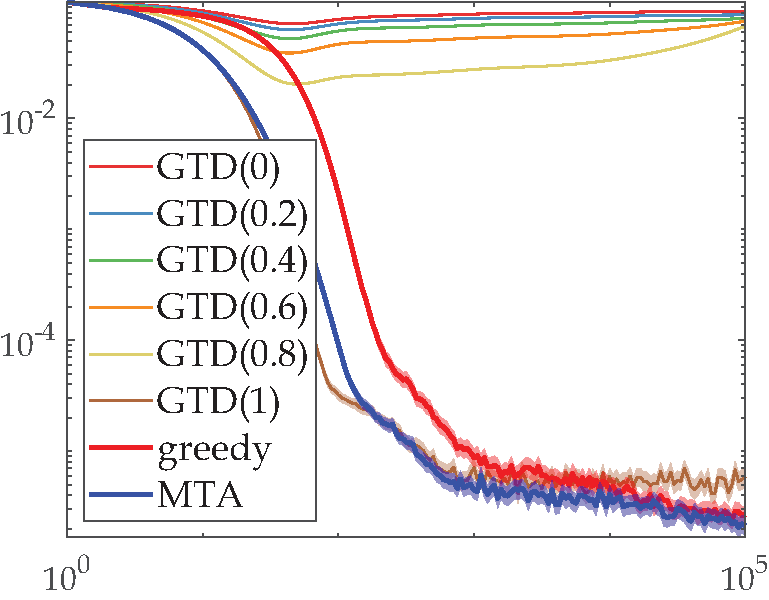
\includegraphics[width=0.45\textwidth]{fig_ringworld_on_1_value.pdf}}
\hfill
\subfloat[$\pi_{l}\!=b_{l}\!=\!0.25$]{
\captionsetup{justification = centering}
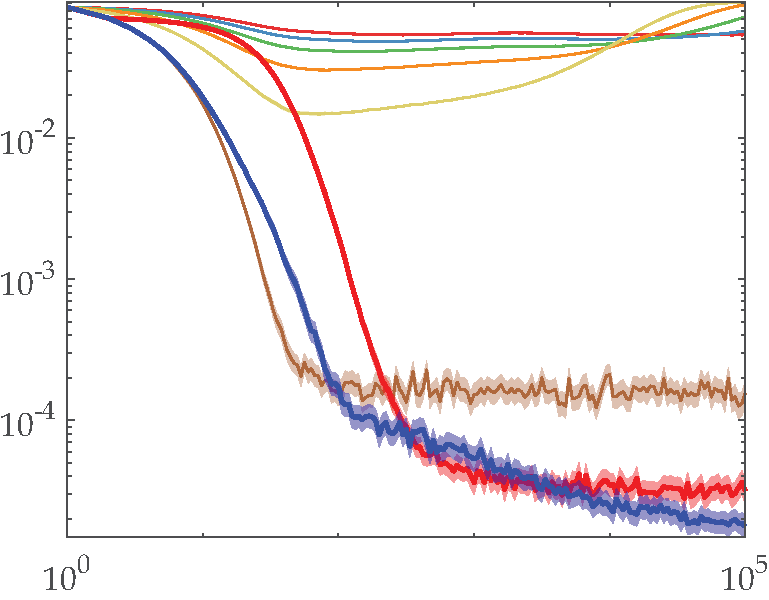
\includegraphics[width=0.45\textwidth]{fig_ringworld_on_2_value.pdf}}
\hfill
\subfloat[$\pi_{l}\!=b_{l}\!=\!0.4$]{
\captionsetup{justification = centering}
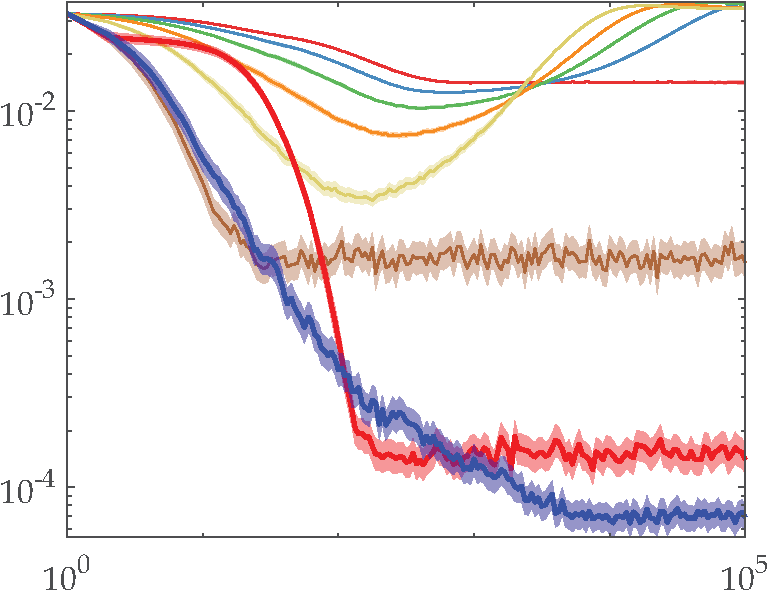
\includegraphics[width=0.45\textwidth]{fig_ringworld_on_3_value.pdf}}
\end{adjustwidth}
\caption{\small On-policy tests on $\gamma = 0.95$ ringworlds.}
\label{fig:ringworld_on}
\end{figure*}

\subsection{$\lambda$ Curves for Tests}
MTA compared to the greedy algorithm: sometimes $\lambda$ converges to zero quickly; Sometimes it bounces and stay relatively high and sometimes it chatters. We think this is a good sign since we are optimizing $\Lambda$ slowly and one $\lambda$ changes along with the changes of the others.
% http://web.mit.edu/jnt/www/Papers/J063-97-bvr-td.pdf
\begin{figure*}
\centering
\begin{adjustwidth}{-1.2in}{-1.2in}
\subfloat[$\pi_{l}\!=\!0.05$, $b_{l}\!=\!0.15$]{
\captionsetup{justification = centering}
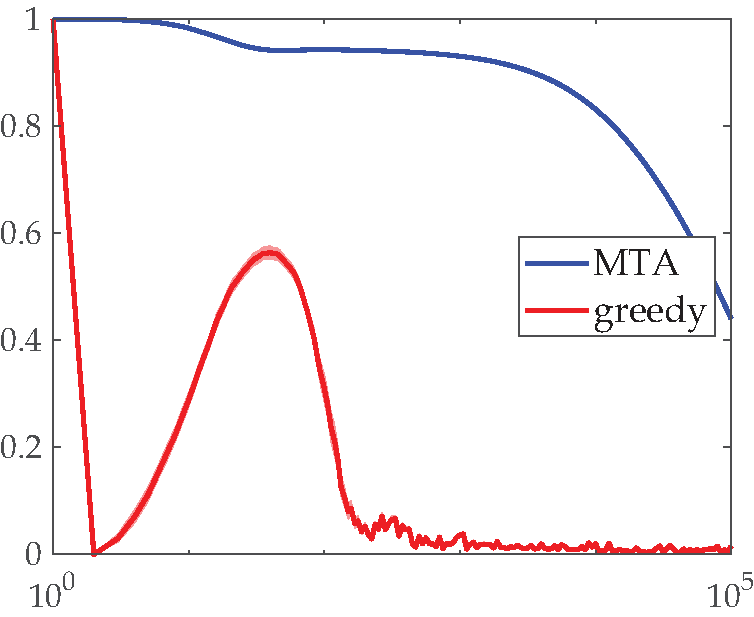
\includegraphics[width=0.45\textwidth]{fig_ringworld_off_1_lambda.pdf}}
\hfill
\subfloat[$\pi_{l}\!=\!0.25$, $b_{l}\!=\!0.33$]{
\captionsetup{justification = centering}
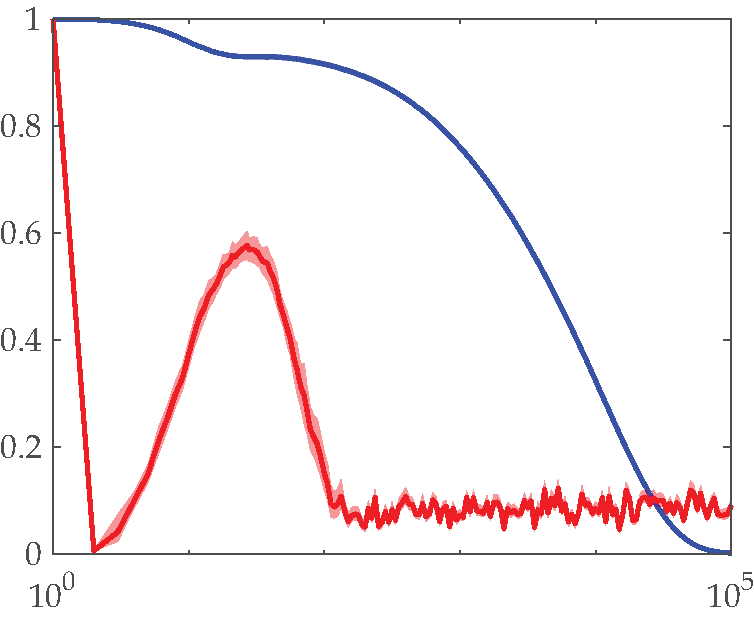
\includegraphics[width=0.45\textwidth]{fig_ringworld_off_2_lambda.pdf}}
\hfill
\subfloat[$\pi_{l}\!=\!0.4$, $b_{l}\!=\!0.5$]{
\captionsetup{justification = centering}
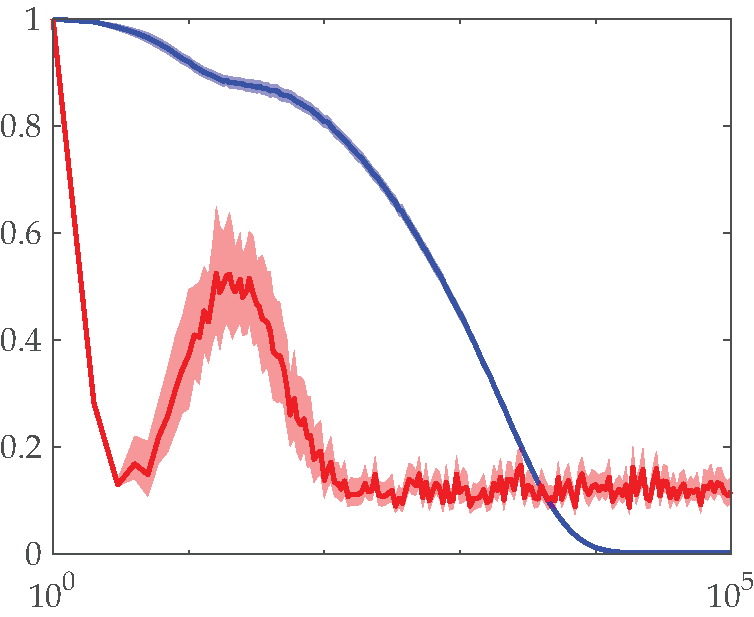
\includegraphics[width=0.45\textwidth]{fig_ringworld_off_3_lambda.pdf}}

\subfloat[$\pi_{l}\!=b_{l}\!=\!0.05$]{
\captionsetup{justification = centering}
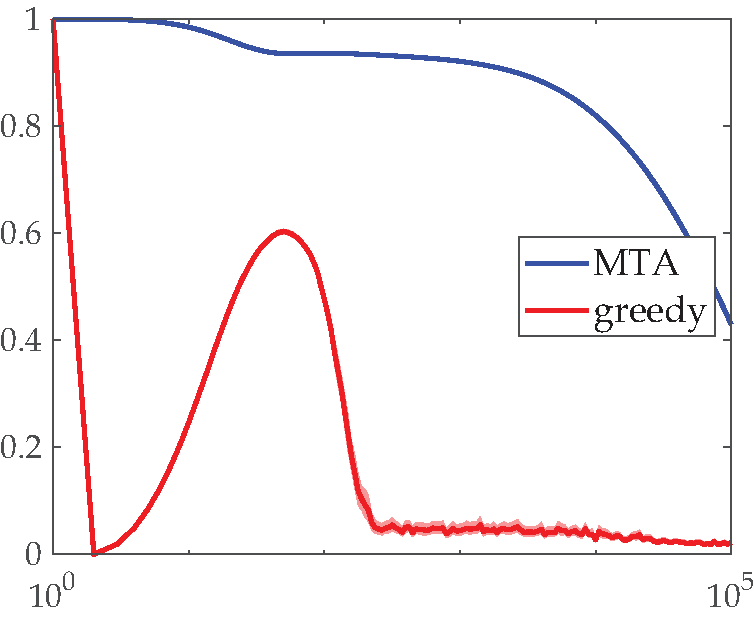
\includegraphics[width=0.45\textwidth]{fig_ringworld_on_1_lambda.pdf}}
\hfill
\subfloat[$\pi_{l}\!=b_{l}\!=\!0.25$]{
\captionsetup{justification = centering}
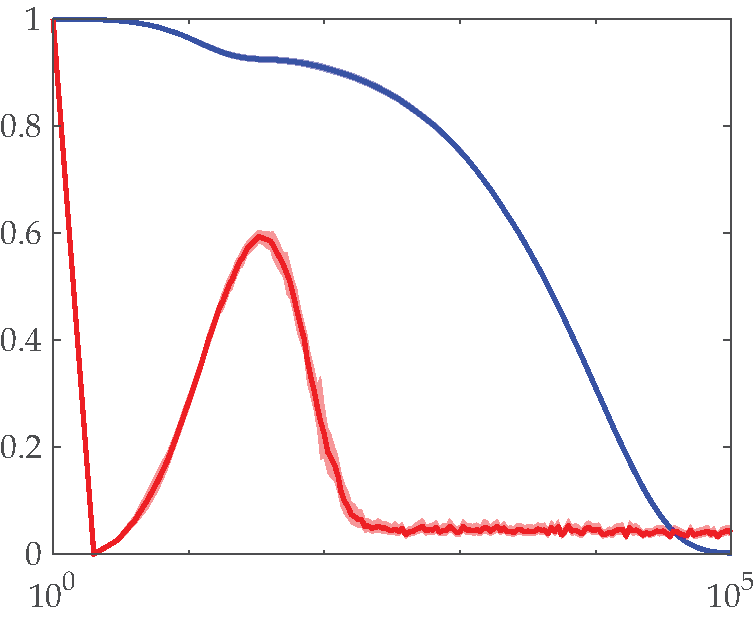
\includegraphics[width=0.45\textwidth]{fig_ringworld_on_2_lambda.pdf}}
\hfill
\subfloat[$\pi_{l}\!=b_{l}\!=\!0.4$]{
\captionsetup{justification = centering}
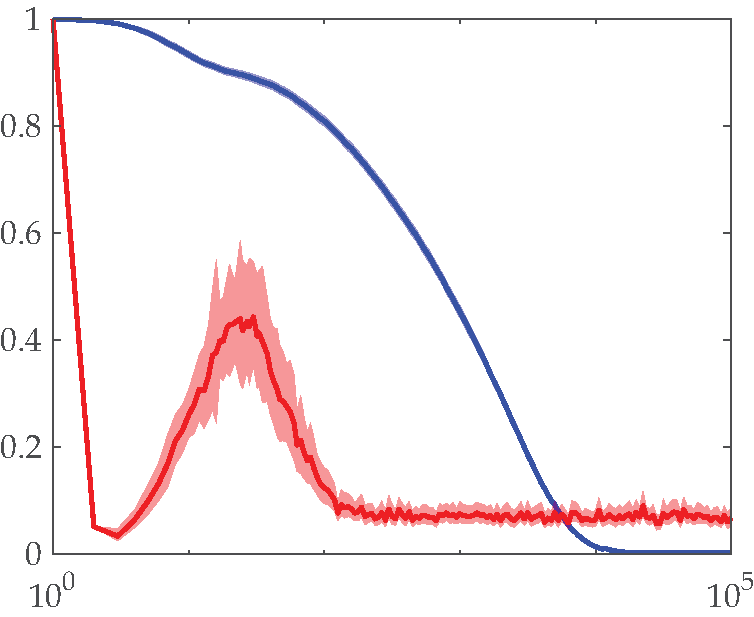
\includegraphics[width=0.45\textwidth]{fig_ringworld_on_3_lambda.pdf}}
\end{adjustwidth}
\caption{\small $\lambda(s_0)$ on $\gamma = 0.95$ ringworlds.}
\label{fig:ringworld_lambda}
\end{figure*}
% http://web.mit.edu/jnt/www/Papers/J063-97-bvr-td.pdf